\chapter{Métodos Actor Critic}%
\label{cha:métodos_actor_critic}

\lecture{6}{2020-06-14}{Actor Critic}

\section{Mejorando Polocy Gradient con un crítico}%
\label{sec:mejorando_polocy_gradient_con_un_crítico}

Se pretende encontrar una mejor estimación de $\hat{Q}_{i,t} = \sum_{t'=t}^T
r(s_{i,t'},a_{i,t'})$. Lo que se quiere es tener una media de varias $\hat{Q}$, lo que lo
acerca más a su esperanza y reduce su varianza.

\begin{align}
\hat { Q } _ { i , t } \approx \sum _ { t ^ { \prime } = t } ^ { T } E _ { \pi _ { \theta } } [ r ( s _ { t ^ { \prime } } , a _ { t ^ { \prime } } ) | s _ { t } , a _ { t } ]
\end{align}

En cuanto al \textit{baseline}, se coge como la media de todas las recompensas
obtenidas:
\begin{align}
    b_t = \frac{1}{N} \sum_i Q(s_{i,t},a_{i,t})
\end{align}

También se puede usar un \textit{baseline} que dependa del estado, ya que se puede demostrar que
el bias sigue siendo 0.
\begin{align}
V ( s _ { t } ) = E _ { a _ { t } \sim \pi _ { \theta } ( a _ { t } | s _ { t } ) } [ Q ( s _ { t } , a _ { t } ) ]
\end{align}

Por lo que el algoritmo Policy Gradient con estas modificaciones queda como:
\begin{align}
\nabla _ { \theta } J ( \theta ) \approx \frac { 1 } { N } \sum _ { i = 1 } ^ { N } \sum _ { t = 1 } ^ { T } \nabla _ { \theta } \operatorname { log } \pi _ { \theta } ( a _ { i , t } | s _ { i , t } ) ( Q ( s _ { i , t } , a _ { i , t } ) - V ( s _ { i , t } ) )
\end{align}

La expresión $ Q ( s _ { i , t } , a _ { i , t } ) - V ( s _ { i , t } ) $ significa cuánto
mejor es una acción que la media de las acciones que se pueden tomar en ese estado, y se
denomina como \textit{advantage}.

\textbf{Recordatorio.}

\begin{align}
    Q ^ { \pi } ( s _ { t } , a _ { t } ) &= \sum _ { t ^ { \prime } = t } ^ { T } E _ { \pi _ {
\theta } } [ r ( s _ { t ^ { \prime } } , a _ { t ^ { \prime } } ) | s _ { t } , a _ { t } ] :
\text { recompensa total tomando } a _ { t } \text { en } s _ { t }\\
            V ^ { \pi } ( s _ { t } ) &= E _ { a _ { t } \sim \pi _ { \theta } ( a _ { t } | s _ { t } ) } [ Q
            ^ { \pi } ( s _ { t } , a _ { t } ) ]: \text{ recompensa total de } s_t\\
            A ^ { \pi } ( s _ { t } , a _ { t } ) &= Q ^ { \pi } ( s _ { t } , a _ { t } ) - V ^ { \pi } ( s _
{ t } ) : \text { cuánto mejor es } a _ { t }\\
\end{align}

Por lo que se puede escribir el algoritmo de la siguiente forma (el cual tendrá una varianza
baja):
\begin{align}
            \nabla _ { \theta } J ( \theta ) &\approx \frac { 1 } { N } \sum _ { i = 1 } ^ { N } \sum _ { t =
1 } ^ { T } \nabla _ { \theta } \operatorname { log } \pi _ { \theta } ( a _ { i , t } | s _ { i
, t } ) A ^ { \pi } ( s _ { i , t } , a _ { i , t } )
\end{align}

Cuanto mejor sea la estimación de $A^\pi$, la varianza será menor.

En el algoritmo con \textit{baseline} que se vio en el tema anterior la estimación del
\textit{advantage} no es del todo buena. No tiene bias, pero tiene una varianza mayor que
si se calculase una $b$ para cada estado.

Lo que se puede hacer es tener una red neuronal que estime una de estas tres: $Q^\pi, V^\pi, A^\pi$. 
Cada una tiene sus ventajas e inconvenientes, por ejemplo $Q^\pi$ es más difícil de
aprender que  $V^\pi$ ya que depende de  $s_t$ y  $a_t$, o  $A^\pi$ es mucho más dependiente de
la política que las otras dos opciones. El algoritmo Actor Critic clásico estima  $V^\pi$.

\begin{align}
    Q ^ { \pi } ( s _ { t } , a _ { t } ) &= r ( s _ { t } , a _ { t } ) + \sum _ { t ^ { \prime } = t
+ 1 } ^ { T } E _ { \pi _ { \theta } } [ r ( s _ { t ^ { \prime } } , a _ { t ^ { \prime } } ) |
s _ { t } , a _ { t } ]\\
&= r ( s _ { t } , a _ { t } ) + E _ { s _ { t + 1 } \sim p ( s _ { t + 1 } | s _ { t } , a _ { t
} ) } [ V ^ { \pi } ( s _ { t + 1 } ) ]\\
&\approx r ( s _ { t } , a _ { t } ) + V ^ { \pi } ( s _ { t + 1 } )
\end{align}

El último paso es una aproximación tomando una muestra, esto se puede ahcer ya que la función
valor tiene en cuenta todas las actualizaciones hechas previamente. Por lo que el advantage
queda como:
\begin{align}
A ^ { \pi } ( s _ { t } , a _ { t } ) \approx r ( s _ { t } , a _ { t } ) + V ^ { \pi } ( s _ { t + 1 } ) - V ^ { \pi } ( s _ { t } )
\end{align}

Por tanto se define una red neuronal que dado $s$ estima un valor $\hat{V}^\pi(s)$.
Esta red tiene como parámetros $\phi$ (ya que la red que estima las acciones tiene los parámetros
representados con $\theta$).

\section{El problema de evaluación de la política}%
\label{sec:el_problema_de_evaluación_de_la_política}

Consiste en dada una política, calcular los valores de los estados. Para estimar los valores,
se tiene que ejecutar la políticas numerosas veces en el entorno (Monte Carlo).

\begin{align}
V ^ { \pi } ( s _ { t } ) \approx \sum _ { t ^ { \prime } = t } ^ { T } r ( s _ { t ^ { \prime } } , a _ { t ^ { \prime } } )
\end{align}

Si se pudiese retroceder en el tiempo (que en el mundo real no se puede), se podrían estimar de
la siguiente manera, que daría mejores resultados:

\begin{align}
V ^ { \pi } ( s _ { t } ) \approx \frac { 1 } { N } \sum _ { i = 1 } ^ { N } \sum _ { t ^ { \prime } = t } ^ { T } r ( s _ { t ^ { \prime } } , a _ { t ^ { \prime } } )
\end{align}

Pero al no ser siempre posible, la estimación de 4.14 sigue siendo bastante buena. Esto se debe
a que al trabajar con un aproximador (red neuronal), no se puede pretender tener valores
exactos para cada estado, sino que estados similares acabarán con valores similares.

Para entrenar al crítico, se crean los datos de entrenamiento para hacer aprendizaje
supervisado:

\begin{align}
\{ ( s _ { i , t } , \sum _ { t ^ { \prime } = t } ^ { T } r ( s _ { i , t ^ { \prime } } , a _ { i , t ^ { \prime } } ) ) \}
\end{align}

Y se hace la regresión:
\begin{align}
L ( \phi ) = \frac { 1 } { 2 } \sum _ { i } \| \hat { V } _ { \phi } ^ { \pi } ( s _ { i } ) - y _ { i } \| ^ { 2 }
\end{align}

¿Esto se puede mejorar? Sí. Se puede hacer un rollout de la siguiente manera:
\begin{align}
y _ { i , t } = \sum _ { t ^ { \prime } = t } ^ { T } E _ { \pi _ { \theta } } [ r ( s _ { t ^ {
\prime } } , a _ { t ^ { \prime } } ) | s _ { i , t } ] \approx r ( s _ { i , t } , a _ { i , t }
) + V ^ { \pi } ( s _ { i , t + 1 } ) \approx r ( s _ { i , t } , a _ { i , t } ) + \hat { V } _
{ \phi } ^ { \pi } ( s _ { i , t + 1})
\end{align}

Se puede ver que en el último paso lo que se hace es coger la estimación de $\hat{V}^\pi$
obtenida por nuestra red neuronal, que es exactamente lo que estamos intentando
optimizar. Esto produce un valor ligeramente erróneo, pero reduce la varianza ya que ese
valor ha sido calculado tras varios pasos por ese estado. Al hacer esto, los datos de
entrenamiento pasan a ser:
\begin{align}
\{ ( s _ { i , t } , r ( s _ { i , t } , a _ { i , t } ) + \hat { V } _ { \phi } ^ { \pi } ( s _ { i , t + 1 } ) ) \}
\end{align}

Estos datos tienen bias, pero son una estimación mejor porque reducen la varianza. Cuando se
hace esto se le suele llamar \textit{bootstraping}.

Reordenando las ideas anteriores, se define el algoritmo Actor Critic:
\begin{algorithm}
    \caption{Actor-Critic}
    \label{alg:actor-critic}
    \While{seguir con el entrenamiento}{
        Muestrear $\{s_i,a_i\}$ de $\pi_\theta(a|s)$\\
        Optimizar  $\hat{V}^\pi_\phi(s)$ a la suma de recompensas muestreadas\\
        Evaluar
        $\hat{A}^\pi(s_i,a_i)=r(s_i,a_i)+\hat{V}^\pi_\phi(s'_i)-\hat{V}^\pi_\phi(s_i)$\\
        $\nabla _ { \theta } J ( \theta ) \approx \sum _ { i } \nabla _ { \theta } \operatorname
        { log } \pi _ { \theta } ( a _ { i } | s _ { i } ) \hat { A } ^ { \pi } ( s _ { i } , a _
        { i } )$\\
        $\theta \gets \theta + \alpha\nabla_\theta J(\theta)$
    }
\end{algorithm}

\section{Factores de descuento}%
\label{sec:factores_de_descuento}

En el caso de que el algoritmo \ref{alg:actor-critic} se use en un entorno sin horizonte y en
el que las recompensas no dependan del tiempo, por ejemplo recompensa 1 siempre mientras el
agente siga vivo, $V^\pi$ puede llegar a diverger.\\ Para arreglar esto se pueden usar factores
de descuento.

Para esto, se hace la asunción de que las recompensas es mejor obtenerlas cuanto antes.
Matemáticamente esto se formula así:
\begin{align}
y _ { i , t } \approx r ( s _ { i , t } , a _ { i , t } ) + \gamma \hat { V } _ { \phi } ^ { \pi } ( s _ { i , t + 1 } )
\end{align}

Donde $\gamma$ es el factor de descuento y está entre 0 y 1 (normalmente 0.99 funciona bien).

Al introducir el factor de descuento en un MDP, lo que se está haciendo efectivamente es
crear otro MDP en el que hay otro estado nuevo. Este estado nuevo se puede considerar como 'la
muerte'. Ahora el agente puede 'morir' con probabilidad $(1-\gamma)$ desde cualquier estado.

\begin{figure}[htpb]
	\centering
	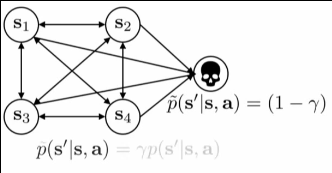
\includegraphics[width=0.3\linewidth]{figures/2020-06-14-114943_332x173_scrot.png}
\end{figure}

Por ejemplo, la aplicación de esto a Policy Gradient (Monte Carlo) puede quedar de estas formas:
\begin{itemize}
    \item Opción 1
        \begin{align}
\nabla _ { \theta } J ( \theta ) \approx \frac { 1 } { N } \sum _ { i = 1 } ^ { N } \sum _ { t = 1 } ^ { T } \nabla _ { \theta } \operatorname { log } \pi _ { \theta } ( a _ { i , t } | s _ { i , t } ) ( \sum _ { t ^ { \prime } = t } ^ { T } \gamma ^ { t ^ { \prime } - t } r ( s _ { i , t ^ { \prime } } , a _ { i , t ^ { \prime } } ) )
        \end{align}
    \item Opción 2: Usarlo antes de aplicar el truco de la causalidad
        (sección \ref{sec:reducir_la_varianza_causalidad})
        \begin{align}
\nabla _ { \theta } J ( \theta ) \approx \frac { 1 } { N } \sum _ { i = 1 } ^ { N } ( \sum _ { t = 1 } ^ { T } \nabla _ { \theta } \operatorname { log } \pi _ { \theta } ( a _ { i , t } | s _ { i , t } ) ) ( \sum _ { t = 1 } ^ { T } \gamma ^ { t - 1 } r ( s _ { i , t ^ { \prime } } , a _ { i , t ^ { \prime } } ) )
        \end{align}
\end{itemize}

Estos dos no son lo mismo, calculan gradientes diferentes. Para la opción 1, al introducir el
crítico se queda de la siguiente forma:
\begin{align}
\nabla _ { \theta } J ( \theta ) \approx \frac { 1 } { N } \sum _ { i = 1 } ^ { N } \sum _ { t = 1 } ^ { T } \nabla _ { \theta } \operatorname { log } \pi _ { \theta } ( a _ { i , t } | s _ { i , t } ) ( r ( s _ { i , t } , a _ { i , t } ) + \gamma \hat { V } _ { \phi } ^ { \pi } ( s _ { i , t + 1 } ) - \hat { V } _ { \phi } ^ { \pi } ( s _ { i , t } ) )
\end{align}

En la opción 2, si se aplica causalidad se obtiene la expresión:
\begin{align}
\nabla _ { \theta } J ( \theta ) \approx \frac { 1 } { N } \sum _ { i = 1 } ^ { N } \sum _ { t = 1 } ^ { T } \nabla _ { \theta } \operatorname { log } \pi _ { \theta } ( a _ { i , t } | s _ { i , t } ) ( \sum _ { t ^ { \prime } = t } ^ { T } \gamma ^ { t ^ { \prime } - 1 } r ( s _ { i , t ^ { \prime } } , a _ { i , t ^ { \prime } } ) )
\end{align}

Lo único que cambia con respecto a la opción 1 es el exponente de $\gamma$. Si se reordena,
queda más claro cual es la diferencia con respecto a la opción 1:
\begin{align}
\nabla _ { \theta } J ( \theta ) \approx \frac { 1 } { N } \sum _ { i = 1 } ^ { N } \sum _ { t = 1 } ^ { T } \gamma ^ { t - 1 } \nabla _ { \theta } \operatorname { log } \pi _ { \theta } ( a _ { i , t } | s _ { i , t } ) ( \sum _ { t ^ { \prime } = t } ^ { T } \gamma ^ { t ^ { \prime } - t } r ( s _ { i , t ^ { \prime } } , a _ { i , t ^ { \prime } } ) )
\end{align}

Como se puede ver todo queda multiplicado por $\gamma^{t-1}$. Lo que hace que los pasos tomados
más tarde importen menos que los tomados antes para el gradiente. La opción 2 es la opción
correcta si se quiere mantener la misma representación de un MDP con el estado de 'muerte'.
Pero en la práctica se suele usar la opción 1, que no resuelve el MDP con el estado de 'muerte'.

La opción 1 en su lugar está optimizando un problema de frontera infinita pero previniendo las
sumas infinitas. Estas sumas infinitas hacen que la varianza crezca mucho, por lo que se puede
interpretar que $\gamma$ lo que hace es intercambiar varianza por la introducción de bias
(valores bajos de $\gamma$ producen menos varianza pero más bias).

Demostración: \textit{Bias in natural actor-critic algorithms. Philip Thomas. ICML 2014}.

\section{El algoritmo Actor Critic}%
\label{sec:el_algoritmo_actor_critic}

Con descuento, se los algoritmos actor-critic quedan:

\begin{algorithm}
    \caption{Batch Actor-Critic con descuento}
    \label{alg:actor-critic-batch-desc}
    \While{seguir con el entrenamiento}{
        Muestrear $\{s_i,a_i\}$ de $\pi_\theta(a|s)$\\
        Optimizar  $\hat{V}^\pi_\phi(s)$ a la suma de recompensas muestreadas\\
        Evaluar
        $\hat{A}^\pi(s_i,a_i)=r(s_i,a_i)+\gamma\hat{V}^\pi_\phi(s'_i)-\hat{V}^\pi_\phi(s_i)$\\
        $\nabla _ { \theta } J ( \theta ) \approx \sum _ { i } \nabla _ { \theta } \operatorname
        { log } \pi _ { \theta } ( a _ { i } | s _ { i } ) \hat { A } ^ { \pi } ( s _ { i } , a _
        { i } )$\\
        $\theta \gets \theta + \alpha\nabla_\theta J(\theta)$
    }
\end{algorithm}

Se puede derivar una versión \textit{online}. Con Policy Gradients se necesita una
trayectoria completa para estimar el gradiente. Pero con Actor-Critic esto no hace falta, se
puede ir estimando cada paso que se toma.

\begin{algorithm}
    \caption{Online Actor-Critic}
    \label{alg:cont-actor-critic}
    \While{se siga entrenando}{
        Tomar accion $a \sim \pi_\theta(a|s)$, tomar  $(s,a,s',r)$\\
        Actualizar  $\hat{V}^\pi_\phi$ usando el objetivo
        $r+\gamma\hat{V}^\pi_\phi(s')$\\
        Evaluar $ \hat{A}^\pi(s,a) = r(s,a) + \gamma\hat{V}^\pi_\phi(s') -
        \hat{V}^\pi_\phi(s)$\\
        $\nabla _ { \theta } J ( \theta ) \approx \nabla _ { \theta } \operatorname { log } \pi _
        { \theta } ( a | s ) \hat { A } ^ { \pi } ( s , a )$\\
        $\theta \gets \theta + \alpha\nabla_\theta J(\theta)$
    }
\end{algorithm}

El algoritmo \ref{alg:cont-actor-critic} aplicado así no funciona, hay que aplicar algunos ajustes.

\subsection{Diseño de la arquitectura}%
\label{sub:diseño_de_la_arquitectura}

Hay varias formas de crear las redes neuronales para las estimaciones:
\begin{itemize}
    \item Dos redes separadas:
        \begin{itemize}
            \item Es más estable y simple
            \item Como desventaja, no se comparten características entre el actor y el crítico,
                por lo que se tiene que aprender desde 0 en ambos.
        \end{itemize}
\begin{figure}[htpb]
	\centering
	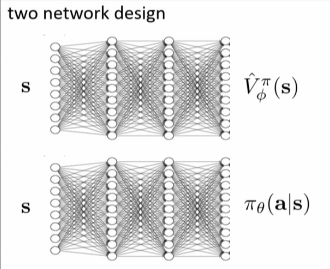
\includegraphics[width=0.4\linewidth]{figures/2020-06-14-123008_330x269_scrot.png}
\end{figure}
    \item Red compartida
    \begin{itemize}
        \item Se comparten los pesos, la desventaja es que se tiene que optimizar dos
            objetivos lo que puede hacer que un gradiente pese más que el otro.
    \end{itemize}
\begin{figure}[htpb]
	\centering
	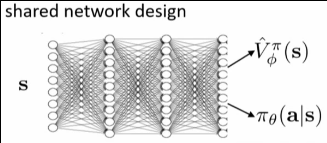
\includegraphics[width=0.4\linewidth]{figures/2020-06-14-123202_327x143_scrot.png}
\end{figure}
\end{itemize}

\subsection{Online Actor-Critic en la práctica}%
\label{sub:online_actor_critic_en_la_práctica}

El problema comentado en el algoritmo \ref{alg:cont-actor-critic} hace referencia a que en
el caso de entrenar de forma contínua se tiene un batch de tamaño 1. Esto es mala idea hasta en
aprendizaje supervisado, lo que se puede hacer es tener a varios agentes interactuando de
manera paralela y recoger un batch a partir de las observaciones de cada uno de ellos. 

Una forma de hacer esto es con \textit{synchronized parallel actror-critic}, donde se obtiene un
batch, se actualiza $\theta$ y así sucesivamente.

También se puede implementar \textit{asynchronous parallel actor-critic}. Donde los parámetros
están guardados en un servidor y las distintas instancias se comunican con él cuando lo
necesitan.

\begin{figure}[htpb]
	\centering
	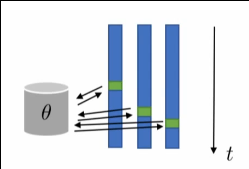
\includegraphics[width=0.3\linewidth]{figures/2020-06-14-123924_249x169_scrot.png}
\end{figure}

El caso asíncrono suele ir más rápido, por eso se usa más en la práctica. Lo único paralelo son
las simulaciones.

Cabe recordar que esto no se hace para que el algoritmo entrene más rápido, sino para que
funcione. Si se quiere entrenar más rápido, habría que tener también a varios trabajadores
paralelos calculando gradientes.

\subsection{Críticos como baselines dependientes del estado}%
\label{sub:críticos_como_baselines_dependientes_del_estado}

En Actor-Critic, el Critic se usa para estimar el \textit{advantage}. Aunque esto reduce la
varianza, incrementa el bias por dos posibles razones:
\begin{itemize}
    \item Puede ser que se use el critic anterior
    \item El critic da valores erróneos
\end{itemize}

Por otro lado, Policy Gradients (que es un método Monte Carlo), no tiene bias, pero padece de
una alta varianza.

Se puede calcular $\hat{V}^\pi_\phi$ para que sea $b$ y hacer que la varianza se reduzca
manteniendo el bias a 0.

\begin{align}
\nabla _ { \theta } J ( \theta ) \approx \frac { 1 } { N } \sum _ { i = 1 } ^ { N } \sum _ { t = 1 } ^ { T } \nabla _ { \theta } \operatorname { log } \pi _ { \theta } ( a _ { i , t } | s _ { i , t } ) ( ( \sum _ { t ^ { \prime } = t } ^ { T } \gamma ^ { t ^ { \prime } - t } r ( s _ { i , t ^ { \prime } } , a _ { i , t ^ { \prime } } ) ) - \hat { V } _ { \phi } ^ { \pi } ( s _ { i , t } ) )
\end{align}

Si se quisiera hacer lo mismo pero con los valores de las acciones en vez del estado, se tiene
que sumar la esperanza de Q ya que su media no es 0. La esperanza se puede obtener aproximada
(Para más información mirar \textit{Q-prop} de Gu, et. al).
\begin{align}
\nabla _ { \theta } J ( \theta ) \approx \frac { 1 } { N } \sum _ { i = 1 } ^ { N } \sum _ { t = 1 } ^ { T } \nabla _ { \theta } \operatorname { log } \pi _ { \theta } ( a _ { i , t } | s _ { i , t } ) ( \hat { Q } _ { i , t } - Q _ { \phi } ^ { \pi } ( s _ { i , t } , a _ { i , t } ) ) + \frac { 1 } { N } \sum _ { i = 1 } ^ { N } \sum _ { t = 1 } ^ { T } \nabla _ { \theta } E _ { a \sim \pi _ { \theta } ( a _ { t } | s _ { i , t } ) } [ Q _ { \phi } ^ { \pi } ( s _ { i , t } , a _ { t } ) ]
\end{align}

\section{Elegibility traces y n-step returns}%
\label{sec:elegibility_traces_y_n_step_returns}

Como se ha visto, se tienen las dos aproximaciones:
\begin{figure}[H]
	\centering
	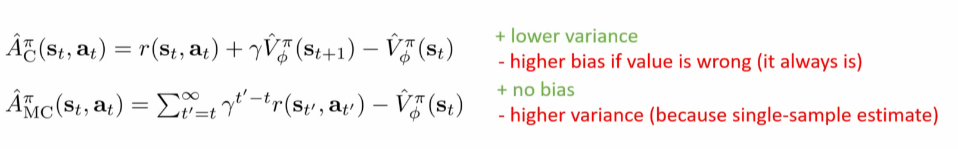
\includegraphics[width=1.0\linewidth]{figures/2020-06-14-125640_958x149_scrot.png}
\end{figure}

Se pretende buscar una forma de obtener las ventajas de los dos métodos y controlar la
relación bias/varianza.

Cuando se proyecta una trayectoria en el futuro, la varianza de los estados inmediatos es baja,
pero la de tiempos lejanos es muy alta. Por ejemplo, si me levanto mañana se que tengo que ir al
trabajo en un 99\% pero puede ser que me ponga malo con un 1\%. Sin embargo, si pienso en mi
futuro profesional dentro de 30 años lo más seguro es que me equivoque.

Monte Carlo es útil para obtener valores de tiempos cercanos, pero inútiles a largo plazo. Y los
basados en valor son más o menos al revés. Su bias puede ser perjudicial al comienzo pero
en el futuro su baja varianza hace que hagan predicciones más o menos buenas.

Lo que se puede hacer es elegir donde cortar:

\begin{figure}[htpb]
	\centering
	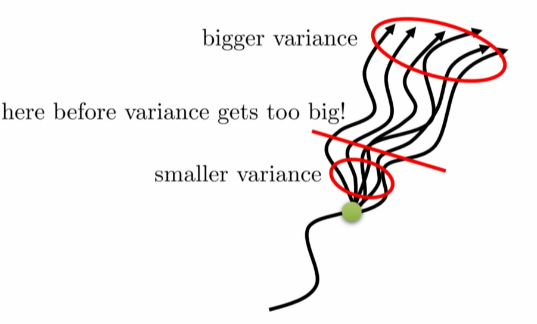
\includegraphics[width=0.5\linewidth]{figures/2020-06-14-130429_537x324_scrot.png}
\end{figure}

Lo que se puede hacer es tener una estimación que considere los $n$ pasos más recientes:
\begin{align}
\hat { A } _ { n } ^ { \pi } ( s _ { t } , a _ { t } ) = \sum _ { t ^ { \prime } = t } ^ { t + n } \gamma ^ { t ^ { \prime } - t } r ( s _ { t ^ { \prime } } , a _ { t ^ { \prime } } ) - \hat { V } _ { \phi } ^ { \pi } ( s _ { t } )
\end{align}

Esto puede tener sentido en entornos muy estocásticos, donde predecir el futuro no tenga
mucho sentido. Pero lo normal es dejar a $\hat{V}_\phi^\pi$ para predecir el futuro.

\begin{align}
    \label{eq:an}
\hat { A } _ { n } ^ { \pi } ( s _ { t } , a _ { t } ) = \sum _ { t ^ { \prime } = t } ^ { t + n
} \gamma ^ { t ^ { \prime } - t } r ( s _ { t ^ { \prime } } , a _ { t ^ { \prime } } ) - \hat {
V } _ { \phi } ^ { \pi } ( s _ { t } ) + \gamma^n \hat{V}_\phi^\pi(s_{t+n})
\end{align}

Normalmente elegir $n>1$ da mejores resultados.

\subsection{Generalized Advantage Estimation}%
\label{sub:generalized_advantage_estimation}

En vez de elegir una $n$ donde cortar en la ecuación \ref{eq:an}, se puede calcular el
\textit{advantage} como una combinación ponderada de infinitos \textit{n-step returns}.

\begin{align}
\hat { A } _ { GAE } ^ { \pi } ( s _ { t } , a _ { t } ) = \sum _ { n = 1 } ^ { \infty } w _ { n } \hat { A } _ { n } ^ { \pi } ( s _ { t } , a _ { t } )
\end{align}

Los pesos interesa escogerlos de tal forma que los \textit{n-steps} donde la n es menor tengan
más preferencia, por lo que se escoge un decrecimiento exponencial:
\begin{align}
    w_n \propto \lambda^{n-1}
\end{align}

Por lo que queda:
\begin{align}
\hat { A } _ { GAE } ^ { \pi } ( s _ { t } , a _ { t } ) = r ( s _ { t } , a _ { t } ) + \gamma (
( 1 - \lambda ) \hat { V } _ { \phi } ^ { \pi } ( s _ { t + 1 } ) + \lambda ( r ( s _ { t + 1 } ,
a _ { t + 1 } ) + \gamma ( ( 1 - \lambda )\hat{V}_\phi^\pi(s_{t+2})\ldots
\end{align}

Que se puede simplificar a:
\begin{align}
\hat { A } _ { GAE } ^ { \pi } ( s _ { t } , a _ { t } ) = \sum _ { t ^ { \prime } = t } ^ { \infty } ( \gamma \lambda ) ^ { t ^ { \prime } - t } \delta _ { t ^ { \prime } }
\end{align}

Donde $d_t$ es:
 \begin{align}
\delta _ { t ^ { \prime } } = r ( s _ { t ^ { \prime } } , a _ { t ^ { \prime } } ) + \gamma \hat { V } _ { \phi } ^ { \pi } ( s _ { t ^ { \prime } + 1 } ) - \hat { V } _ { \phi } ^ { \pi } ( s _ { t ^ { \prime } } )
\end{align}

Se puede observar que $\gamma$ y $\lambda$ estan juntas como base de la exponencial, por lo que
tienen el mismo significado. Como $\lambda$ se introdujo para reducir la varianza, se
comprueba que se estaba en lo cierto cuando anteriormente en la opción 1 se pensaba que
$\gamma$ reducía la varianza.
